Dado un grafo simple G = ( V , E ) se quiere buscar la solución con un algoritmo exacto al problema de k-PMP, se realiza un algoritmo con la técnica de backtracking para obtener la misma.

\subsection{Desarrollo}

Para comenzar el desarrollo es necesario definir previamente cada una de las estructuras que se utilizan en el mismo. Sabemos que el grafo esta representado por un conjunto de vértices, cada uno de los mismos tiene una etiqueta en este caso es un numero desde $1$ hasta $n$, siendo $n$ la cantidad de vértices del grafo, a su vez tenemos un conjunto de tuplas que representan los ejes en el grafo. Toda esta información la volcamos a una matriz de adyacencias, donde cada posición se tiene 0 si las aristas no están conectadas o el valor del peso del eje en caso que estén conectados.

Una solución, llamada $solFinal$, será representada con un conjunto de $k$ subconjuntos, donde cada uno contendrá las etiquetas de los vértices, disjuntos de a pares (un vertice pertenece a un único subconjunto) y el peso del conjunto será la suma de cada uno de los pesos de los subconjuntos, donde el peso del subconjunto se entienden a la suma de los pesos de las aristas que conecten dos vértices del mismo subconjunto.

Además diremos que una k partición A es mejor que otra B si el peso total es menor, es decir si A es mejor que B entonces $peso(A) < peso(B)$. 

La clave del algoritmo de Backtracking es que explorara de forma recursiva todas las posibles combinaciones de subconjuntos.

en cada llamado recursivo intentara insertar un vértice a la solución que esta armando, en caso de no tener una mejor solución tratara de insertar ese vértice en otro subconjunto que no haya probado, así hasta haber probado todos los subconjuntos y sin ir mas lejos si se realiza este ejercicio estaremos realizando todas las combinaciones de los vértices en los k subconjuntos.	

Nuestro solFinal en principio va a ser el conjunto donde todos los vértices estén en el primer subconjunto.


De la siguiente manera:
\begin{algorithm}
  \begin{algorithmic}[1]\parskip=1mm
 \caption{ backtracking(solParcial,solFinal,numeroVertice,cantidadSubConjuntos)}
 		\STATE{Si Puedo insertar } 
		\STATE{\quad para cada i desde 1 hasta cantidadSubConjuntos: }
 		\STATE{\quad\quad agrego el numeroVertice al subconjunto i en SolParcial}
 		\STATE{\quad\quad backtracking ( solParcial , solFinal, numeroVertice+1,k,adyacencias)}
		\STATE{\quad\quad saco el elemento que agregue al ultimo conjunto}
		\STATE{Si Puedo insertar }   
		\STATE{devuelvo False}
  \end{algorithmic}
  \end{algorithm}


Ahora de esa manera lo único que estamos haciendo es probar todas las combinaciones , pero no estamos quedándonos con la mejor k - partición para esto debemos definir una función que nos diga cuando una solución es mejor que otra y además debemos saber si ya insertamos todos los vértices.

Para lo cual definimos una función que devuelve un numero indicando 0 si inserte todos los vértices llegando a otra solución, luego tengo que ver si es mejor que la que tengo hasta el momento y 1 si tengo que seguir insertando vértices.
Quedándonos de la siguiente manera:

\begin{algorithm}
  \begin{algorithmic}[1]\parskip=1mm
 \caption{numero check(adyacencias, solParcial,solFinal, numeroVertice,cantidadVertices)}
 		\STATE{SI numeroVertice=cantidadDeVertices }   
 		\STATE{\quad devolver 0}
 		\STATE{SI NO}
		\STATE{\quad devolver 1}
  \end{algorithmic}
  \end{algorithm}
    
\begin{algorithm}
  \begin{algorithmic}[1]\parskip=1mm
 \caption{backtracking(solParcial,solFinal,numeroVertice,cantidadSubConjuntos,adyacencias, cantidadVertices)}
 		\STATE{entero resultadoCheck = check(adyacencias,solParcial,solFinal,numeroVertice,cantidadVertices) }   
 		\STATE{si resultadoCheck = 0 }   
 		\STATE{\quad Remplazo mi solFinal por solParcial}
 		\STATE{Si NO}
		\STATE{\quad para cada i desde 1 hasta cantidadSubConjuntos: }
 		\STATE{\quad\quad agrego el numeroVertice al subconjunto i en SolParcial}
 		\STATE{\quad\quad backtracking ( solParcial , solFinal, numeroVertice+1,k,adyacencias)}
		\STATE{\quad\quad saco el elemento que agregue al ultimo conjunto}
		\STATE{devuelvo False}

  \end{algorithmic}
  \end{algorithm}

Con este algoritmo estaremos probando todas las combinaciones de todos los vértices en los k subconjuntos, en cada paso insertamos un vértice a un subconjunto y llamamos a la recursión con el siguiente vértice. una vez que vuelva de la recursión quitara el vértice del conjunto donde lo ingreso y seguirá el ciclo insertándolo en otro subconjunto y llamando a la recursión de nuevo.

\subsection{Podas}
Para mejorar los tiempos del algoritmo es necesario realizar algún tipo de validación intermedia para no probar casos que no nos van a llevar a una solución optima, por ejemplo cuando estamos insertando vértices a la solución que ya tiene mas peso que nuestra mejor solución o cuando nos quedan una cantidad de vértices es menor estricta a la cantidad de subconjuntos vacíos, estas podas son las que realizamos en nuestro algoritmo agregándolas a la función check al Backtracking de la siguiente manera:

\begin{algorithm}
  \begin{algorithmic}[1]\parskip=1mm
 \caption{numero check(adyacencias, solParcial,solFinal, numeroVertice,cantidadVertices)}
 		\STATE{SI peso(solParcial)$ >$ peso(solFinal) }   
 		\STATE{\quad devolver 2}
		\STATE{SI numeroVertice=cantidadDeVertices }   
 		\STATE{\quad devolver 0}
 		\STATE{Si cantidadDeCajasVacias(solParcial)$ >$ cantidadVertices }   
 		\STATE{\quad devolver 2}
		\STATE{devolver 1}
  \end{algorithmic}
  \end{algorithm}
La funcion cantidadDeCajasVacias se fija si algun conjunto no tiene  
 
 \begin{algorithm}
 \begin{algorithmic}[1]\parskip=1mm
 \caption{backtracking(solParcial,solFinal,numeroVertice,cantidadSubConjuntos,adyacencias, cantidadVertices)}
 		\STATE{entero resultadoCheck = check(adyacencias,solParcial,solFinal,numeroVertice,cantidadVertices) }   
 		\STATE{si resultadoCheck = 0 }   
 		\STATE{\quad Remplazo mi solFinal por solParcial}
		\STATE{si resultadoCheck = 2 }   
 		\STATE{\quad devuelvo false porque mi solParcial es peor que mi solFinal o tengo mas cajas vacías que vertices para poner	l}
 		\STATE{Si NO}
		\STATE{\quad para cada i desde 1 hasta cantidadSubConjuntos: }
 		\STATE{\quad\quad agrego el numeroVertice al subconjunto i en SolParcial}
 		\STATE{\quad\quad backtracking ( solParcial , solFinal, numeroVertice+1,k,adyacencias)}
		\STATE{\quad\quad saco el elemento que agregue al ultimo conjunto}
		\STATE{devuelvo False}
  \end{algorithmic}
  \end{algorithm}

De esta manera el algoritmo va a realizar las podas en las llamadas recursivas intermedias antes de insertar todos los vértices descartando casos que no son útiles para llegar  a una solución optima en menor tiempo.

Para improvisar una mejora en la poda al comparar los pesos de nuestras soluciones parcial y final, lo que realizamos es generar otra solución final asignando cada uno de los vértices de manera creciente a cada uno de las k subconjuntos diferentes y si esta otra solución es mejor a la solución que tiene todos los nodos en un solo conjunto la tomamos como solución final para nuestras comparaciones.
De esta manera podrían tomarse otro tipo de soluciones para luego obtener la solución final de menor peso y podar mas ramas del Backtracking.	

\subsection{Complejidad}
Dado que el algoritmo exacto sin las podas prueba todas las soluciones del problema esto hace que sea poco eficiente en terminos de tiempo a comparacion de las heuristicas que iremos viendo a lo largo del informe. Pero conociendo las soluciones que se van a ir armando pueden definirse podas para evitar seguir resolviendo ramas de la solucion que no me van a llevar a una solucion optima o a una solucion que no es mejor que la que ya forme hasta cierto punto.
Dado el algoritmo exacto mostraremos las complejidades de las diferentes partes del mismo para obtener cual seria la complejidad final.

\begin{algorithm}
  \begin{algorithmic}[1]\parskip=1mm
 \caption{numero check(adyacencias, solParcial,solFinal, numeroVertice,cantidadVertices)}
 		\STATE{SI peso(solParcial) > peso(solFinal)  $\mathcal{O}(1)$}   
 		\STATE{\quad devolver 2}
		\STATE{SI numeroVertice=cantidadDeVertices $\mathcal{O}(1)$ }   
 		\STATE{\quad devolver 0}
 		\STATE{Si cantidadDeCajasVacias(solParcial) $>$ cantidadVertices $\mathcal{O}(k)$}   
 		\STATE{\quad devolver 2}
		\STATE{devolver 1}
  \end{algorithmic}
  \end{algorithm}

Para la funcion check la complejidad final sera $\mathcal{O}(1)$ + $\mathcal{O}(1)$ + $\mathcal{O}(k)$ dando como complejidad total $\mathcal{O}(k)$.

\begin{algorithm}
 \begin{algorithmic}[1]\parskip=1mm
 \caption{backtracking(solParcial,solFinal,numeroVertice,cantidadSubConjuntos,adyacencias, cantidadVertices)}
 		\STATE{entero resultadoCheck = check(adyacencias,solParcial,solFinal,numeroVertice,cantidadVertices)$\mathcal{O}(k)$ }   
 		\STATE{si resultadoCheck = 0 $\mathcal{O}(1)$}   
 		\STATE{\quad Remplazo mi solFinal por solParcial $\mathcal{O}(k)$}
		\STATE{si resultadoCheck = 2 $\mathcal{O}(1)$}   
 		\STATE{\quad devuelvo false porque mi solParcial es peor que mi solFinal o tengo mas cajas vacías que vertices para poner $\mathcal{O}(1)$}
 		\STATE{Si NO}
		\STATE{\quad para cada i desde 1 hasta cantidadSubConjuntos: }
 		\STATE{\quad\quad agrego el numeroVertice al subconjunto i en SolParcial}
 		\STATE{\quad\quad backtracking ( solParcial , solFinal, numeroVertice+1,k,adyacencias)}
		\STATE{\quad\quad saco el elemento que agregue al ultimo conjunto}
		\STATE{devuelvo False}
  \end{algorithmic}
  \end{algorithm}

El ciclo de las lineas 7-10 se ejecuta k veces en cada llamado iterativo, cada ves que se llama a la funcion backtracking es por un vertice diferente. 
Para el primer nodo tenemos k conjuntos para probar, luego con el segundo vertice tenemos para cada uno de esos conjuntos donde coloque el primer nodo k alterativas de conjuntos para probar quedandonos $k^2$ combinaciones para esos dos vertices,
para cada una de esas $k^2$ combinaciones tenemos k conjuntos quedando $k^3$ combinaciones, asi seguira en las llamadas recursivas por todos los vertices. Con lo cual con el vertice n tendremos $k^n$ combinaciones para este vertice.

Por lo tanto la complejidad total del algortimo es del orden de $\mathcal{O}(k^n)$ siendo $k$ la cantidad de subconjuntos y $n$ la cantidad de vertices del grafo.

\subsection{Experimentacion}
Para el analisis de este algoritmo se generaron 30 instancias de manera random de grafos completos con vertices entre 1 y 20 elegidos de manera aleatoria mediante un script en python con la funcion randint.
Luego para esas instancias se corrio el algoritmo asignando 5, 10 y 15 subconjuntos para ver como se comportaba el algoritmo, obteniendose como resultado lo siguiente:\\
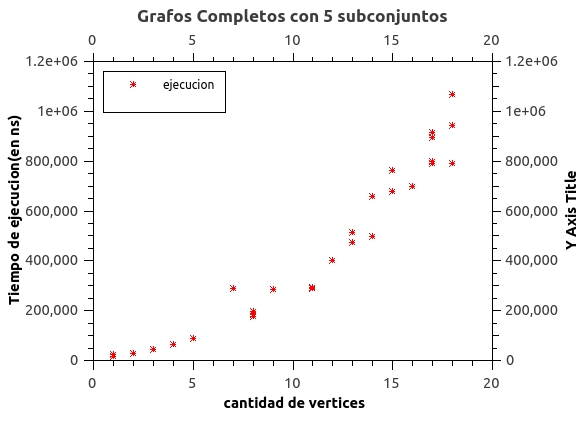
\includegraphics[scale=0.5]{Ej2/k5.jpg}
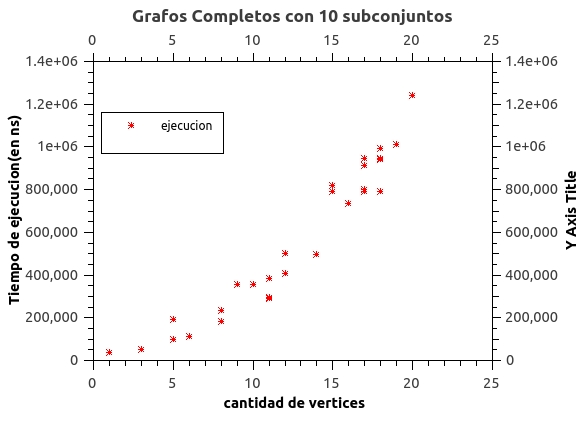
\includegraphics[scale=0.5]{Ej2/k10.jpg}\\
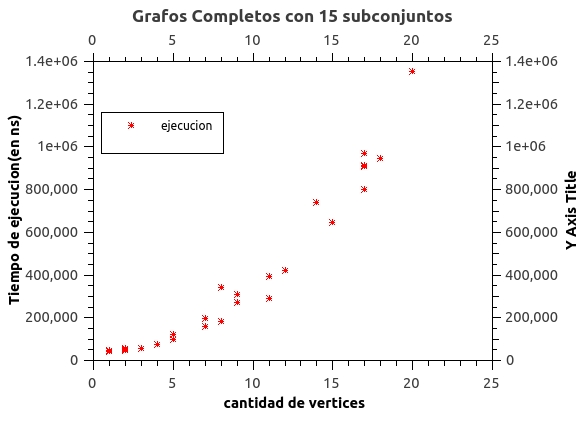
\includegraphics[scale=0.5]{Ej2/k15.jpg}\\

Se puede ver como la curva se hace mas pronunciada al cambiar la cantidad de subconjuntos, con esto se ve que al cambiar el k la complejidad va aumentando de manera exponencial.

Por otro lado realizamos un analisis sobre las podas, para esto primero generamos 30 instancias de grafos para ver como se comportaba el algoritmo con grafos sin aristas, obteniendo el siguiente resultado:\\
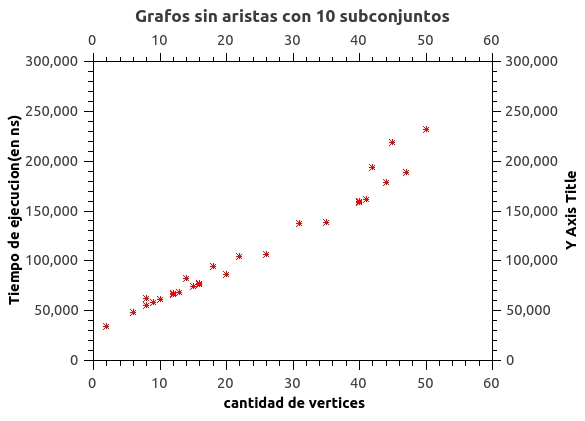
\includegraphics[scale=0.5]{Ej2/sinAristas.jpg}\\
Como puede verse el grafico los tiempos de ejecucion son similares a una lineal, esto se debe a que como la solucion inicial tiene peso 0 ya que no tiene aristas, en cada llamado recursivo se devuelve false porque no se obtiene nada mejor en cuestion de peso del conjunto.
Por otro lado como mencionamos en el desarrollo del algoritmo se agrego una genacion de una solucion inicial alternativa a poner todos los vertices en un solo subconjunto, por lo que realizamos una experimentacion para ver como afectaba la no presencia de esta solucion alternativa, corrimos las mismas instancias de grafos para 15 subconjuntos que corrimos en los priemros test donde se encontraba esta solucion alternativa y obtuvimos lo siguiente:\\
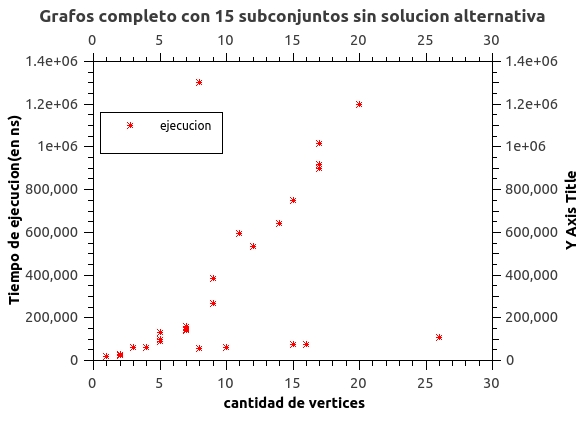
\includegraphics[scale=0.5]{Ej2/sinAlternativa.jpg}\\

Como puede observarse los tiempos empeoran ya que la primera solucion a nuestro problema es el grafo con todos las aristas y esto puede no podar muchas ramas del backtracking que con la solucion alternativa si se estan podando. Concluyedo que podrian mejorar los tiempos si estamos eligiendo una buena solucion inicial.

